\documentclass{book}
\usepackage[utf8]{inputenc}
\usepackage{fullpage}
\usepackage{graphicx}
\usepackage{sansmath}
\usepackage{amsmath}
\usepackage[dutch]{babel}
\usepackage{vub}
\usepackage{hyperref}
\usepackage{float}
\raggedbottom
\let\cleardoublepage\clearpage


% VUB-voorblad configureren
\author{Nicolas Carraggi, Youri Coppens, Christophe Gaethofs, Pieter Meiresone, Sam Van den Vonder, Fernando Suarez, Tim Witters}
\title{Software Project Management Plan}
\subtitle{Software Engineering}
\faculty{Faculteit Ingenieurswetenschappen \& Wetenschappen}
\department{}
\date{Academiejaar 2013-2014}

% VUB huisstijl voor font en kleur == veel mooier dan het standaard (vergeet package bovenaan niet te activeren!!!!)
\color{pantone418}
\renewcommand{\familydefault}{\sfdefault}
\sansmath

\begin{document}
\frontmatter
\makeassignment
\chapter{Versiegeschiedenis}

\begin{table}[htbp]
	\centering
	\caption{Versiegeschiedenis}
	\begin{tabular} {|c|c|c|c|}
	    \hline
		\textbf{Versie} & \textbf{Datum} 	& \textbf{Auteur(s)} & \textbf{Commentaar} \\
		\hline
		1.0	& 30/11/2013	& Sam Van den Vonder & Initi\"{e}le versie \\ \hline
		1.1 & 10/12/2012	& Sam Van den Vonder & Aanpassingen kwaliteitsinspectie \\ \hline
	\end{tabular}
\end{table}
\tableofcontents
\listoffigures
\listoftables

\mainmatter

\chapter{Overzicht}
\section{Samenvatting van het project}
\subsection{Doel, scope en objectieven}
Het doel van dit project is het maken van een webapplicatie die het mogelijk maakt om lessenroosters binnen de universiteit te schedulen. Deze lessenroosters moeten vervolgens door de studenten geraadpleegd kunnen worden. Er is verder specifieke support voor mobiele platformen nodig.
\\
\\
Als projectnaam is gekozen voor ``CalZone'', ge\"{i}spireerd op het feit dat we een zone voor een kalender moeten maken. Het logo is afgebeeld in figuur \ref{fig:logoProject}.
\begin{figure} [H]
    \centering
    
\includegraphics[width = 0.75\textwidth]{Overview/logo_Green_Crop.jpg}
    \caption{Het logo.}
    \label{fig:logoProject}
\end{figure}
%\subsection{Onderstellingen en beperkingen}

\subsection{Project deliverables}
De deliverables voor dit project zijn de volgende:
\begin{itemize}
	\item Functionerende website die voldoet aan de requirements gespecifieerd in het SRS.
	\item Software Project Management Plan (SPMP)
	\item Software Test Plan (STD)
	\item Software Requirements Specification (SRS)
	\item Software Design Document (SDD)
	\item Minutes van alle vergaderingen
	\item Source code en aanverwanten
\end{itemize}
Deze documenten worden in .pdf formaat samen in een enkele zipfile verstuurd via mail. De documenten zijn ook beschikbaar op de GitHub repository. Op het einde van elke iteratie wordt ook de code van het project opgeleverd, deze zit dan in dezelfde zipfile als de documenten. In tabel \ref{tab:kalender} staat de lijst van data waarop de code en de documenten worden opgeleverd. Na elke iteratie volgt een presentatie waar het geleverde werk voor die iteratie wordt gedemonstreert en besproken. 
\begin{table}[H]
  \centering
  \caption{Kalender}
    \begin{tabular}{c|c}
    \textbf{Datum} & \textbf{To Do} \\
    \hline
    Maandag 04/11/2013 & Inleveren SPMP \\
    Vrijdag 15/11/2013 & Eerste versie documenten \\
    Vrijdag 13/12/2013 & Einde iteratie 1: opleveren code en documenten \\
    Woensdag 18/12/2013 & Presentatie \\
    \hline
    \hline
    Dinsdag 04/03/2014 & Einde iteratie 2: opleveren code en documenten \\
    Woensdag 12/03/2014 & Presentatie \\
    Dinsdag 15/04/2014 & Einde iteratie 3: opleveren code en documenten \\
    Woensdag 23/04/2014 & Presentatie \\
    Vrijdag 16/05/2014 & Einde iteratie 4: opleveren code en documenten \\
    Woensdag 21/05/2014 & Finale presentatie \\
    \end{tabular}
  \label{tab:kalender}
\end{table}

Meer gedetailleerde informatie is te vinden in paragraaf \ref{sec:rapportering}.

\section{Evolutie van het SPMP}
De evoluatie van de SPMP zal bijgehouden worden met behulp van een versie geschiedenis in het begin van dit document. Er zullen steeds geplande updates uitgevoerd worden op de tijdsstippen beschreven in tabel \ref{tab:kalender}. 
\\
\\
Deze updates worden uitgevoerd met behulp van de GitHub Repository \cite{GitHubRepository}. Met behulp van GitHub kunnen we met issues werken, en hiervoor telkens een verantwoordelijke aanduiden.
\chapter{Referenties}
\begingroup
\renewcommand{\chapter}[2]{}%
\begin{thebibliography}{99}

    \bibitem{portalWebsite} \emph{Portal Team Website.} \url{http://wilma.vub.ac.be/~se2_1314/website/}
    
    \bibitem{ShareLateX} \emph{ShareLateX.} \url{https://www.sharelatex.com}
    
    \bibitem{GitHubRepository} \emph{GitHub Repository.} \url{https://github.com/CalZoneVUB}
    
    \bibitem{GitHubAPI} \emph{GitHub API.} \url{http://developer.github.com/v3/}
    
    \bibitem{WilmaServer} \emph{Wilma.} \url{http://wilma.vub.ac.be/}
    
    \bibitem{MicrosoftProject} \emph{Microsft Project.} \url{http://office.microsoft.com/nl-be/project/}
    
    \bibitem{DreamsparkVUB} \emph{Microsoft DreamSpark for VUB-Engineering Students.} \url{http://e5.onthehub.com/WebStore/Welcome.aspx?ws=4ec25e81-649b-e011-969d-0030487d8897&vsro=8}
    
    \bibitem{WBSChartPro} \emph{WBS Chart Pro.} \url{http://www.criticaltools.com/wbsmain.htm}
    
    \bibitem{EclipseMetricsPlugin} \emph{Eclipse Metrics Plugin.} \url{http://eclipse-metrics.sourceforge.net/}
    
    \bibitem{VUBHuisstijl} \emph{De huisstijl van de VUB.} \url{http://www.vub.ac.be/home/huisstijl/}

	\bibitem{CocomoI} \emph{COCOMO I.} \url{http://en.wikipedia.org/wiki/COCOMO}
	
	\bibitem{CocomoII} \emph{COCOMO II.} \url{http://csse.usc.edu/tools/COCOMOII.php}
	
	\bibitem{SoftwareEngineeringAModernApproach} \emph{Software Engineering: Modern Approaches.} Eric J. Braude \& Michael E. Bernstein

    \bibitem{Eclipse} \emph{Eclipse.} \url{http://www.eclipse.org}
    
    \bibitem{Javadoc} \emph{Javadoc.} \url{http://www.oracle.com/technetwork/java/javase/documentation/index-jsp-135444.html}

	\bibitem{HendersonSellers} \emph{Henderson-Seller metriek.} \url{http://eclipse-metrics.sourceforge.net/descriptions/pages/cohesion/HendersonSellers.html}
	
	\bibitem{JavaCodeConventions} \emph{Code Conventions for the Java Programming Language} \url{http://www.oracle.com/technetwork/java/codeconv-138413.html}
	
	\bibitem{JavadocConventions} \emph{Javadoc Conventions. } \url{http://www.oracle.com/technetwork/java/javase/documentation/index-137868.html}





\end{thebibliography}


\endgroup
\chapter{Definities}
\begin{table} [H]
    \centering
    \caption{Overzicht van de gebruikte acroniemen.}
\begin{tabular}{l|l}
    Acroniem & Betekenis \\
    \hline
    STD & Software Test Documentation \\
    SRS & Software Requirement Specification \\
    SDD & Software Design Document \\
    SPMP & Software Project Management Plan \\
    GUI & Graphical User Interface
\end{tabular}
\end{table}
\chapter{Project organisatie} \label{chap:ProjectOrganisatie}
\section{Externe interfaces}
Dit project wordt geproduceerd in opdracht van het vak Software Engineering. Communicatie verloopt via mail met Jens Nicolay\footnote{\href{mailto:jnicolay@vub.ac.be}{jnicolay@vub.ac.be}}, Ragnild van Der Straeten\footnote{\href{mailto:rvdstrae@vub.ac.be}{rvdstrae@vub.ac.be}} en Dirk van Deun\footnote{\href{mailto:dirk@dinf.vub.ac.be}{dirk@dinf.vub.ac.be}}. Jens Nicolay en Ragnild van Der Straeten worden gecontacteerd voor functionale zaken, terwijl Dirk van Deun gecontacteerd wordt voor technische zaken betreffende de infrastructuur.

\section{Interne structuur} \label{sec:InterneStructuur}
Voor dit project is er een team van 7 personen. De takenverdeling binnen dit team is als volgt:
\begin{table} [H]
	\centering
	\caption{Takenverdeling.}
	\begin{tabular} {l|cc}
		Rol & Verantwoordelijke & Reserve \\
		\hline
		Project Manager & Pieter & Nicolas \\
		Configuration Manager & Christophe & Tim \\
		Database Manager & Nicolas & Christophe \\
		Quality assurance Manager & Sam & Youri \\
		Requirements Manager & Fernando & Pieter \\
		Design Manager & Youri & Sam \\
		Implementation Manager & Tim & Fernando \\
		\hline
		Webmaster & Christophe & \textbackslash \\
		Secretaris & Fernando & \textbackslash 
	\end{tabular}
	\label{tab:takenverdeling}
\end{table}

Communicatie binnen het team verloopt via de website \cite{portalWebsite}. Hier wordt een soort blog gebruikt door de teamleden. Een teamlid kan een bericht plaatsen en achteraf kan op dit bericht gereageerd worden door andere teamleden. Een voorbeeldinteractie is weergegeven in figuur \ref{fig:communicatieExample}. Verder wordt er gebruik gemaakt van de mailinglijst op wilma om de verschillende teamleden van een notificatie te voorzien bij de aanmaak van een nieuw bericht. 
\begin{figure} [H]
	\centering
	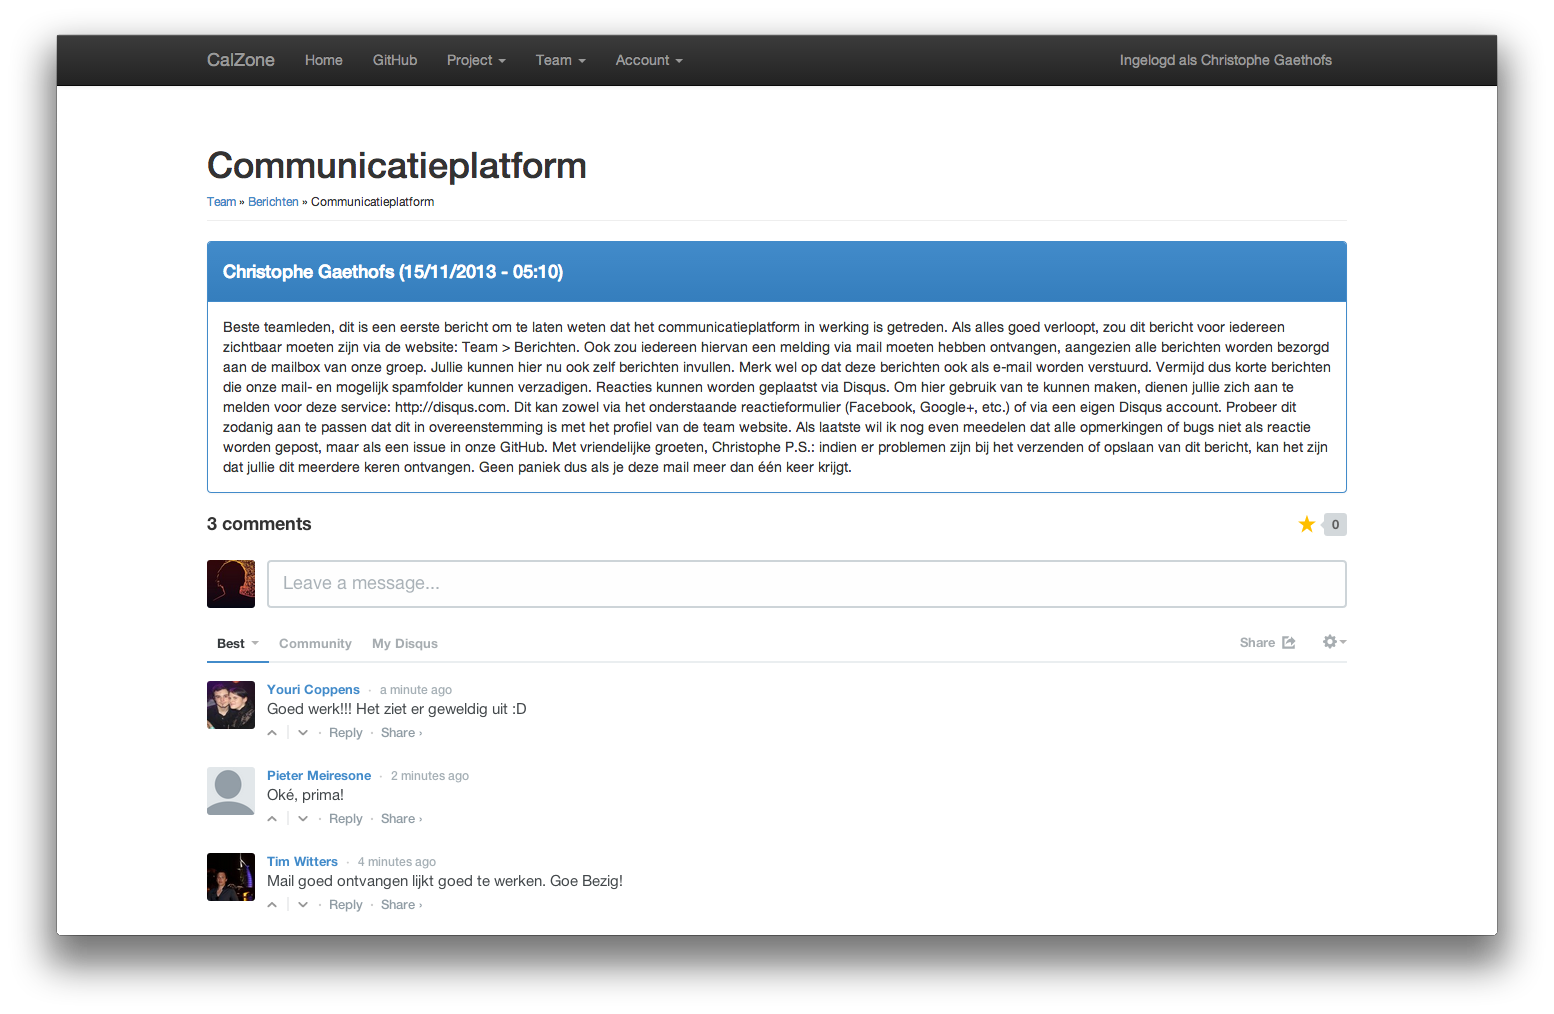
\includegraphics[width = \textwidth]{ProjectOrganization/Communication.png}
	\caption{Communicatie op de team website.}
	\label{fig:communicatieExample}
\end{figure}

\section{Rollen en verantwoordelijkheden}
Elk teamlid is verantwoordelijk voor een functie en reserve van een andere functie (zie tabel \ref{tab:takenverdeling}).Ook speelt elk teamlid een rol in de codering van het systeem. 

Hier volgt een gedetailleerd overzicht van deze functies:
\begin{table} [H]
	\centering
	\caption{Functies.}
	\begin{tabular} {l | p{10cm}}
		Functie & Verantwoordelijkheden \\
		\hline
		Project Manager &  
		\begin{itemize}
		\item Verantwoordelijkheid over SPMP
		\item Opvolging van managers
		\item Zorgt ervoor dat deadlines binnen het team gerespecteerd worden
		\item Ingrijpen waar nodig
		\end{itemize}\\
		\hline
		Configuration Manager &
		\begin{itemize}
		\item Verantwoordelijkheid over SCMP (onderdeel van SPMP)
		\item Keuze software en procedures
		\item Controle van gebruik van software en instellingen.
		\end{itemize}\\
		\hline
		Database Manager &
		\begin{itemize}
		\item Onderhoud en controle database
		\item Onderscheid maken tussen en beheren van test en officiële database
		\end{itemize}\\
		\hline
		Quality Assurance Manager &
		\begin{itemize}
		\item Verantwoordelijkheid over SQAP (onderdeel van SPMP)
		\item Verantwoordelijkheid over STD
		\item Controle en correctie van nauwkeurigheid en styling van code en documenten
		\item Algemene testing van software
		\end{itemize}\\
		\hline
		Requirements Manager &
		\begin{itemize}
		\item Verantwoordelijkheid over SRS
		\item Controle van uitvoering van requirements
		\item Verificatie van uitgewerkte requirements
		\end{itemize}\\
		\hline
		Design Manager &
		\begin{itemize}
		\item Verantwoordelijkheid over SDD
		\item modelleren en architectuur bepalen van het systeem
		\end{itemize}
	\end{tabular}
	\label{tab:functies}
\end{table}
\begin{table} [H]
	\centering
	\caption{Functies (vervolg).}
	\begin{tabular} {l | p{10cm}}
		Functie & Verantwoordelijkheden \\
		\hline
		Implementation Manager &
		\begin{itemize}
		\item Verdelen van system requirements onder de developers
		\item Controle van de progressie van de code
		\item Controle van de uitvoering van het design
		\end{itemize}\\
		\hline
		Webmaster &
		\begin{itemize}
		\item Onderhoud teamwebsite
		\item Onderhoud projectwebsite (die dat de gebruikers van het systeem gebruiken).
		\end{itemize}\\
		\hline
		Secretaris &
		\begin{itemize}
		\item Verslagen van vergaderingen bijhouden
		\end{itemize}\\
	\end{tabular}
\end{table}
\chapter{Management process}
\section{Project start plan} \label{sec:ProjectStartPlan}
Voor het project management zal er gebruikt worden van Microsoft Project \cite{MicrosoftProject}. Een licentie valt gratis te verkrijgen via Microsoft Dreamspark for VUB Students \cite{DreamsparkVUB}. M.b.v. Microsoft Project zullen er Gantt charts gegenereerd worden. Voor Work Breakdown Structures zal er gebruik worden gemaaakt van WBS Chart Pro \cite{WBSChartPro}. Hiervan is een demo-versie verkrijgbaar die voldoende functionaliteit biedt. WBS Chart Pro kan op basis van een Microsoft Project file onmiddelijk een WBS genereren.
\\
\\
In deze paragraaf bespreken we de verwachte kost van het project. Voor de kostberekening maken we gebruik van het COCOMO I model \cite{CocomoI}. Ondanks dat het COCOMO I model reeds verouderd is t.o.v. COCOMO II \cite{CocomoII}, verkiezen we toch COCOMO I. De reden hiervoor is dat COCOMO II afhant van veel inputparameters. Vermits we hiervoor weinig tot geen ervaring hebben, verkiezen we COCOMO I dat slechts afhangt van 2 inputparameters. Bij COCOMO I zijn de vrije parameters het project type en aantal lijnen code. Als type project moeten we kiezen tussen ``simple'', ``semidetached'' en ``embedded''. We kiezen hierin voor het type ``semidetached''. Dit weerspiegelt goed de huidige situatie van ons team. De omvang van ons team is aan de grote kant en er zijn veel onbekende factoren in dit project (zie ook \ref{sec:risicoManagementPlan}). We berekenen dan de effort $E$ uitgedrukt in persoonsmaanden (pm) als
\begin{equation*}
	E = a*KLOC^b
\end{equation*}
Hierbij zijn $a$ en $b$ constanten gegeven door het COCOMO I-model. Voor ons is het interessanter om naar de werkuren te kijken i.p.v. het aantal persoonsmaanden. Volgens de COCOMO standaard bevat \'{e}\'{e}n werkmaand 152 uren.  De benodigde tijd ($T$) is dan
\begin{equation*}
	T = 152\frac{u}{pm}*E
\end{equation*}
Hierbij wordt T uitgedrukt in uren. Uit de tabellen van het COCOMO-model volgt dat $a = 3.0$ en $b = 1.12$. Verder schatten we in dat dit project een totale omvang zal hebben van 10KLOC. Dit geeft dan:
\begin{equation*}
	T = 152*3.0*10^{1.12} \approx 6011u 
\end{equation*}
Vermits ons team uit 7 personen bestaat, geeft dit per persoon een tijdsduur van:
\begin{equation*}
	T_{persoon} \approx 859u
\end{equation*}
Het is evident dat een werklast van $859u$ per persoon niet haalbaar is. Dit hoge resultaat is waarschijnlijk het gevolg van de onbetrouwbare methode COCOMO I. Tegenwoordig zijn er meer tools beschikbaar (waaronder GitHub) die de productiviteit sterk verhogen. 
\\
\\
Op basis van de Gantt-chart die zal opgesteld worden in paragraaf \ref{sec:workplan} bekomen we een meer realistische schatting van 
\begin{equation*}
	T_{persoon} \approx 300u
\end{equation*}
\section{Werk plan} \label{sec:workplan}
\subsection{Activiteiten}
Het project bestaat uit volgende activiteiten\footnote{In volgende versies van het SPMP komen hier nog verscheidene activiteiten bij.}, weergegeven als een work breakdown structure in figuur \ref{fig:workbreakdownstructure}. De activiteiten in de WBS komen overeen met de gegroepeerde requirements die in het SRS-document en website te vinden zijn.
\begin{figure} [H]
    \centering
    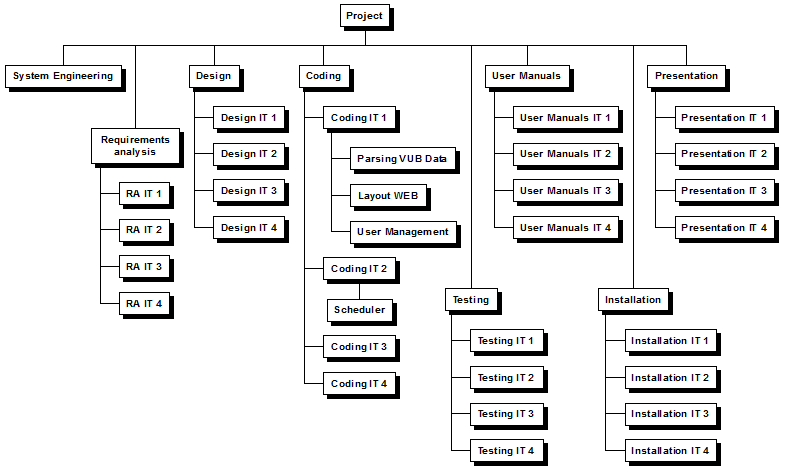
\includegraphics[width = \textwidth]{ManagerialProcess/WBSChart.png}
    \caption{Work breakdown structure.}
	\label{fig:workbreakdownstructure}
\end{figure}
Voor de eerste iteratie is de work breakdown structure weergegeven in figuur \ref{fig:wbsIteratie1}.
\begin{figure} [H]
	\centering
	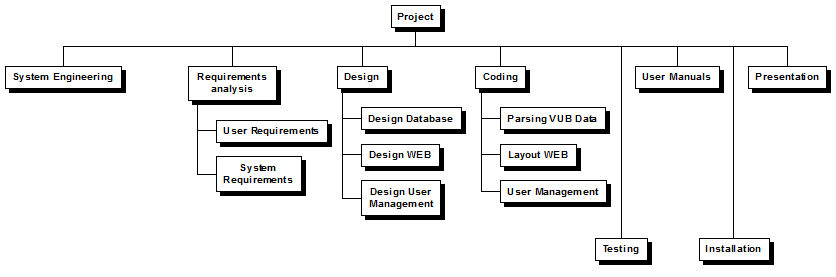
\includegraphics[width = \textwidth]{ManagerialProcess/WBSChartIteratie1.png}
	\caption{Work breakdown structure van iteratie 1.}
	\label{fig:wbsIteratie1}
\end{figure}
In de volgende versies van de SPMP zullen de work breakdown structures van de volgende iteraties worden weergegeven.
\subsection{Planning}
In tabel \ref{tab:ActivityDependenciesIteratie1} is een overzicht weergegeven van de verschillende activiteiten gedurende iteratie 1. Hierbij zijn ook de afhankelijkheden weergegeven tussen deze activiteiten. Op basis van deze tabel kunnen we een Gantt chart opstellen en het kritisch pad bepalen.
\begin{table} [H]
	\centering
	\caption{Activiteiten van de eerste iteratie en afhankelijkheden.}
	\begin{tabular} {l|l|c|c}
		Activiteit ID & Activiteit Naam & Tijdsduur (in dagen) & Afhankelijkheden \\
		\hline
		1 	& System Engineering 		& 28 & \\
		2 	& Requirements Analysis 	& 21 & \\
		2.1 & User Requirements 		& 10 & \\
		2.2 & System Requirements 		& 11 & 2.1 \\
		3 	& Design 					& 5 & 2 \\
		3.1 & Design User Management 	& 5 & \\
		4 	& Coding 					& 21 & \\
		4.1 & Infrastructure onderzoeken & 7 & 2\\
		4.2 & User Management			& 14 & 3, 4.1  \\
		4.2.1 & Frond End 		 		& 14 & \\
		4.2.2 & Back End				& 14 & \\
		5 	& Testing 					& 7 & 4.2 - 7 dagen \\
		6 	& User manuals 				& 3 & 4 \\
		7 	& Installation 				& 1 & 5,6 \\
		8 	& Presentation 				& 3 & 7	
	\end{tabular}
	\label{tab:ActivityDependenciesIteratie1}
\end{table}
Op basis van tabel \ref{tab:ActivityDependenciesIteratie1} bekomen we de Gantt chart voor iteratie 1 weergegeven in figuur \ref{fig:GantChartIT1}. Het kritisch pad is weergegeven in het rood. Hierbij is nog rekening met extra constraints:
\begin{itemize}
	\item Het project is gestart op 15 oktober 2013.
	\item De activiteit ``Requirements Analysis'' kan niet vroeger beginnen dan 24 oktober 2013.
	\item De activiteit ``Installation'' mag niet later eindigen dan 13 december 2013 (zie tabel \ref{tab:kalender}).
	\item De activiteit ``Presentation'' mag niet later eindigen dan 18 december 2013 (zie tabel \ref{tab:kalender}).
\end{itemize}
Op figuur \ref{fig:GantChartIT1} is er te zien dat er nog enkele dagen marge zijn op het einde van iteratie 1. Het kritisch pad mag dus enkele dagen vertraging oplopen.

\begin{landscape}
	\begin{figure} [H]
		\centering
		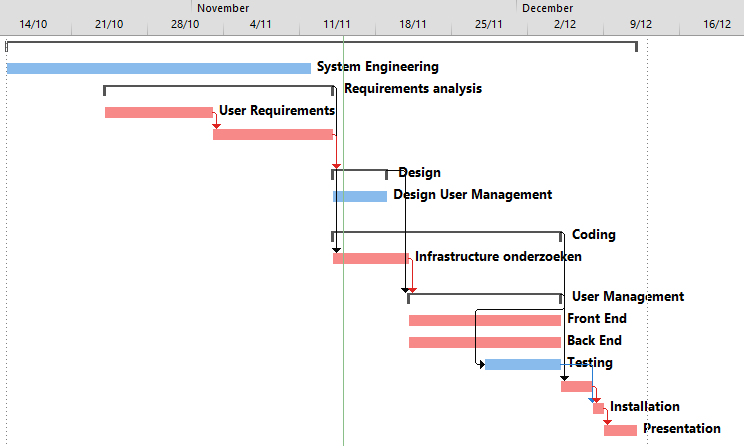
\includegraphics[width = 1.35\textwidth]{ManagerialProcess/GanttChartIT1.png}	
		\caption{Gantt chart voor iteratie 1.}
		\label{fig:GantChartIT1}
	\end{figure}
\end{landscape}


%\subsection{Middelen}
%This subclause of the SPMP shall provide a detailed itemization of the resources allocated to each major work activity in the project work breakdown structure. Resources shall include the numbers and required skill levels of personnel for each work activity. Resource allocation may include, as appropriate, personnel by skill level and factors such as computing resources, software tools, special testing and simulation facilities, and administrative support. A separate line item should be provided for each type of resource for each work activity. A summary of resource requirements for the various work activities should be collected from the work packages of the work breakdown structure and presented in tabular form.
%Voor de design-activiteiten zal er gebruik worden gemaakt van een UML Designer \footnote{De specifieke tool die we gaan gebruiken is nog onder overleg.}. Het coderen zal gebeuren in Eclipse. 

\section{Controle plan}
\subsection{Requirements controle} \label{RequirementsControlPlan}
Er is een requirements dashboard beschikbaar dat een overzicht weergeeft van alle requirements en hun status per iteratie (done, busy, planned, deferred, ... ). Hierbij worden telkens de belangrijkste statistieken per requirement weergegeven (percentage afgewerkt indien bezig, duurtijd implementatie indien klaar, aantal unit tests, ... ). Het onderhoud van het requirements dashboard wordt verzorgd door de Configuration Manager.
\\
\\
Op de website van het team \cite{portalWebsite} is er een pagina beschikbaar die het mogelijk maakt om zaken te rapporteren, en veranderingen door te voeren met betrekkeing tot de SRS. Het is aan de Requirements Manager om ervoor te zorgen dat de verschillende requirements-ID's stabiel blijven. Indien nodig overlegt de Requirements Manager met de Project Manager over eventuele invloed op de planning wanneer er wijzigingen plaatsvinden aan het SRS.

\subsection{Planning controle} \label{sec:PlanningControle}
Voor het opvolgen en schatten van de planning wordt gebruik gemaakt van milestones op GitHub.  Voor elke milestone wordt een verantwoordelijke aangesteld. De vooruitgang t.o.v. elke deadline zal gecontroleerd worden door de bijhorende verantwoordelijke en de Project Manager. Bovendien zal ook de progressie wekelijks op de vergadering besproken worden. Indien de actuele vooruitgang niet overeenkomt met de geplande vooruitgang, kunnen volgende maatregelen genomen worden:
\begin{itemize}
	\item Planning herbekijken.
	\item Teams herindelen.
	\item Sancties voor de verantwoordelijke indien de actuele vooruitgang lager ligt door nalatigheid. Sancties worden vastgelegd door de rest van het team.
\end{itemize} 

\subsection{Budget controle}
Op de website van het team \cite{portalWebsite} wordt er gebruik gemaakt worden van een time tracking tool die het mogelijk maakt een gedetailleerd logboek bij te houden van de reeds uitgevoerde activiteiten. Op basis hiervan kunnen we dan de ``kost'' berekenen van het project. 
\\
\\
De tijdsregistratie wordt uitgevoerd bij het be\"{e}ndigen van elke werkdag. Hierbij wordt telkens opgegeven aan welke activiteit men gewerkt heeft (een overzicht van de verschillende activiteiten bevindt zich in sectie \ref{sec:workplan}).

\subsection{Kwaliteitscontrole}
Ook de kwaliteit zal opgevolgd worden met behulp van de website. De Quality Assurance Manager zal verantwoordelijk zijn voor de kwaliteitspagina op de website.

\subsection{Rapportering} \label{sec:rapportering}
In tabel \ref{tab:kalender} worden de deliverables voor dit project weergegeven. Hierrond worden volgende afspraken gemaakt:
\begin{itemize}
\item Alle documenten en source code (inclusief unit tests) worden per mail aangeleverd als een enkele zipfile, met als naam se2-iterM, waarbij M het nummer van de iteratie is (voor eerste versie van documenten geldt M = 0). De aanlevering gebeurt ten laatste voor 9u00 ’s ochtends op de dag van de deadline (zie tabel \ref{tab:kalender}).
\item Alle documenten en source code worden worden overeenkomstig getagd/gebranchd (se2-iterM) in de GitHub repository.
\item Andere artefacten (zoals executables) worden apart aangeleverd (direct, of via een link, in de opleveringsmail) en vermelden duidelijk de overeenkomstige iteratie in de bestandsnaam.
\item De mail van de oplevering bevat een bondig overzicht (lijstje) van wat er precies opgeleverd
wordt.
\end{itemize}
Voor het verspreiden van de resultaten zal ook gebruik worden gemaakt van de website. 
\begin{itemize}
\item Opgeleverde documenten, source code en andere artefacten moeten publiekelijk en overzichtelijk beschikbaar zijn.
\item Het opleveren van documenten en code per iteratie houdt in dat ten laatste op die welbepaalde dag (zie tabel \ref{tab:kalender}) de site ook up-to-date wordt gebracht.
\end{itemize}
Een presentatie duurt een half uur per groep en wordt ingevuld door 2 sprekers. Alle groepsleden moeten minimum \'{e}\'{e}n keer presenteren. De volgende zaken worden besproken of gedemonstreerd:
\begin{itemize}
\item een demo van de toegevoegde functionaliteit ten opzichte van de vorige iteratie
\item analyse van de ontmoete obstakels en de genomen beslissingen
\item bespreking van de functionaliteiten die aan bod zullen komen in de volgende iteratie
\item bespreking van eventuele obstakels, risico’s, etc. in de volgende iteratie
\item overzicht van de architectuur en design van de applicatie
\item bespreking van de statistieken zoals de tijd per taak en per persoon en van de eventuele vertragingen (plus oplossingen om deze zo klein mogelijk te houden en te vermijden in de toekomst)
\end{itemize}

\subsection{Metriek verzamelingsplan} \label{sec:Metrics}
Metrieken zullen verzameld worden met behulp van de Eclipse Metrics Plugin \cite{EclipseMetricsPlugin}. Er zullen metrieken op methodenniveau en klassenniveau verzameld worden. Op methodenniveau verzamelen we volgende metrieken:
\begin{enumerate}
	\item Cyclomatic Complexity.
	\item Aantal statements
	\item Aantal levels.
	\item Aantal lokale variabelen in de scope.
	\item Aantal parameters.
	\item Feature envy
\end{enumerate}
Op klassenniveau verzamelen we volgende metrieken:
\begin{enumerate}
	\item Efferent Couplings.
	\item Aantal attributen.
	\item Complexiteit
	\item Cohesie tussen de verschillende methodes.
\end{enumerate}
Een gedetailleerde uitleg over deze metrieken is te vinden in bijlage \ref{chap:Metrics}.
\\
\\
De Eclipse Metrics Plugin verzamelt automatisch metrieken bij elk compile process (eens geconfigureerd). Deze worden dan geexporteerd naar een XML-file die vervolgens wordt ingelezen door de website.
\\
\\
Verzamelde metrieken zullen op de webpagina van het team gevisualiseerd worden. De metrieken worden verzameld tijdens de activiteiten waar er gecodeerd wordt. Bij de start van het coderen zullen er wekelijks metrieken verzameld worden. In de laatste week van coderen worden er dagelijks metrieken verzameld, hierdoor kan er refactoring plaatsvinden die de kwaliteit van de code verhoogt.

\section{Risico management plan} \label{sec:risicoManagementPlan}
In deze paragraaf zullen de verschillende risico's verbonden aan dit project besproken worden. In paragraaf \ref{sec:riskPriority} zullen deze risico's geprioritiseerd worden. Om de risico's te kunnen prioritiseren zullen we gebruiken maken van 3 parameters:
\begin{itemize}
	\item 
		De kans $p$ waarmee dit risico kan voorkomen. Hierbij is $ p \in \{1, 2, \ldots , 10\} $. Verder betekent $p = 1$ dat het risico niet kan voorkomen en $p = 10$ dat het risico met zekerheid voorkomt.
	\item 
		De impact $i$ op het project wanneer het risico werkelijkheid wordt. Hierbij is $ i \in \{1, 2, \ldots , 10\} $. Verder betekent $i = 1$ een impact op het project die minimaal is en $i = 10$ een impact die maximaal is.
	\item 
		De kost $c$ die het risico heeft op het project om het probleem op te lossen. Hierbij is $ c \in \{1, 2, \ldots , 10\} $. Hierbij betekent $c = 1$ een lage kostprijs, terwijl $c=10$ een hoge kostprijs betekent. Bij een hoge kostprijs zal de prioriteit van het risico lager gesteld worden, vermits het dan beter kan zijn om pas het risico weg te werken wanneer het voorkomt. Hiermee worden grote onnodige kosten vermeden.
		
\end{itemize}
\subsection{Project risico's}
\subsubsection{Niet-realistische Planning}
In paragraaf \ref{sec:ProjectStartPlan} is de werkduur geschat met het COCOMO I-model. Hier werd reeds duidelijk dat de geschatte tijdsduur enorm hoog ligt. Dit zorgt voor een grote druk op de planning.
\\
\\
Om de vooropgestelde deadlines (zie tabel \ref{tab:kalender}) te bereiken dient men dus voldoende tijd vrij te maken. Het zwaartepunt van het academiejaar van de verschillende groepsleden ligt bij de meeste groepsleden in het eerste semester. Het grootste risico in verband met planning ligt dus vooral bij de eerste iteratie. Dit kan het best vermeden worden door gebruik te maken van interne deadlines en de progressie op te volgen tijdens de wekelijkske teammeetings. Dit is besproken in paragraaf \ref{sec:PlanningControle}.
\\
\\
We karakteriseren dit risico m.b.v. volgende parameters:
\begin{align*}
	p &= 8\\
	i &= 8\\
	c &= 2
\end{align*}

\subsubsection{Communicatieprobleem}
Bij een team van zeven personen is communicatie essentieel. Indien er geen bijzondere maatregelen worden genomen, zal deze snel verkeerd lopen.
\\
\\
Als oplossing hiervoor wordt er reeds een mailinglijst aangeleverd door VUB. Omdat wij deze niet overzichtelijk genoeg vinden, hebben wij zelf een communicatieplatform ontwikkeld op onze website. De werking verloopt als een blog waarbij de teamleaden een bericht kunnen plaatsen en vervolgens hierop kunnen reageren. Bij elk nieuw bericht worden de teamleden van een notificatie voorzien. Dit is ook besproken in paragraaf \ref{sec:InterneStructuur}.
\\
\\
De implementatie hiervan is niet triviaal en vraagt de nodige investering. Wij verwachten echter dat de ``return on investment'' groot zal zijn. Samengevat:
\begin{align*}
	p &= 10\\
	i &= 8\\
	c &= 8
\end{align*}

\subsubsection{Meningsverschillen}
Bij het werken in teamverband is het onvermijdelijk dat er meningsverschillen optreden tussen verscheidene groepsleden. We maken een onderscheid tussen volgende menigsverschillen:
\begin{itemize}
	\item Functioneel: Meningsveschillen waarvan de uitkomst bepalend is voor de uiteindelijke werking van het programma.
	\item Niet-functioneel: Meningsverschillen waarvan de uitkomst niet bepalend is voor de uiteindelijke werking van het programma. Bijvoorbeeld de communicatiemethode, meningsveschillen over interne deadlines, persoonlijke conflicten tussen teamleden, ...
\end{itemize}
Verder kunnen we ook nog onderscheid maken tussen kleine en grote meningsverschillen. Al deze types worden opgelost op een verschillende manier, weergegeven in tabel \ref{tab:meningsverschillen}. De `kost' voor het oplossen van het risico is dus minimaal.
\begin{table} [H]
	\centering
	\caption{Oplossingen voor de verschillende meningsconflicten.}
	\begin{tabular} {l|ll}
					& Functioneel 								& Niet-functioneel \\
			\hline
			Groot 	& Meeting met team, vervolgens stemming		& Behandeld door de verantwoordelijke \\ 
			& & van dit onderwerp \\
			Klein 	& Project Manager							& Behandeld door de verantwoordelijke \\
			& & van dit onderwerp
	\end{tabular}
	\label{tab:meningsverschillen}
\end{table}
We karakteriseren dit risico m.b.v. volgende parameters:
\begin{align*}
	p &= 10\\
	i &= 3\\
	c &= 2
\end{align*}

\subsection{Technische risico's}
\subsubsection{Gebrek aan ervaring in de implementatie-technologie}
Hiervoor wordt er gekeken naar de programmeertalen die gebruikt worden tijdens dit project (zie sectie \ref{sec:languages}). Een overzicht van de aanwezige kwaliteiten is zichtbaar in tabel \ref{tab:skilllevel}. Wat opvalt is dat er van elks kwaliteiten aanwezig zijn, maar er zijn ook de nodige aandachtspunten. Zo is bijvoorbeeld de ervaring in Java en JavaScript beperkt.

\begin{table} [htbp]
	\centering
  	\caption{Ervaring van de verschillende teamleden.}
    \begin{tabular}{c|ccccl}
  		  	& Java 	& JavaScript & HTML \textbackslash CSS 		& SQL 	& Opmerkingen \\
  		  	\hline
  		  	Christophe & -	& ++ 		& ++ 		& ++ & \shortstack{ Reeds ervaring opgedaan \\ in de bedrijfswereld} \\
  		  	Youri & + & - & - & ++ & \shortstack{Voorkeur voor logica, \\ A.I. en modeleren.} \\
  		  	Nicolas & + & - & + & ++ & Voorkeur voor back end \\
  		  	Tim & - & - & + & ++ & \shortstack{Reeds ervaring in C++ en \\ andere programmeerprojecten} \\
  		  	Sam & + & - & + & ++ & \\
  		  	Fernando & - & - & + & ++ & Voorkeur voor design \\
  		  	Pieter & ++ & + & + & + & \shortstack{Reeds ervaring opgedaan \\ in de bedrijfswereld}
    \end{tabular}
  	\label{tab:skilllevel}
\end{table}
Omdat de implementatie-technologie opgelegd wordt, is het gebruik maken van andere frameworks, programmeertalen, ... geen optie. Hierdoor zullen we gebruik maken van workshops. Hiermee gaan we de ervaringen van de verschillende teamleden op elkaar overbrengen. Een workshop wordt georganiseerd door een teamlid die zijn kennis en ervaringen over een bepaalt framework, programmeertaal, ... uiteenzet gedurende 30 \`{a} 60 minuten. Volgende workshops zijn reeds gepland:
\begin{itemize}
	\item GitHub (door Christophe)
	\item Java (door Pieter)
\end{itemize}
Doordat we gebruik maken van korte workshops, zou de invloed van deze workshops op de planning minimaal zijn. We karakteriseren dit risico m.b.v. volgende parameters:
\begin{align*}
	p &= 8\\
	i &= 8\\
	c &= 4
\end{align*}

\subsubsection{Gebrekkige performantie}
Het hoofddoel van dit project is het maken van een scheduler. Het is uiteraard gewenst dat het schedulen vlot verloopt. Vanwege de complexiteit van dit onderwerp zal er ook de nodige aandacht besteedt moeten worden aan de performantie van de scheduler.
\\
\\
Dit zal gemonitored worden met behulp van benchmarks. Indien er tekortkomingen ontdekt worden, zullen de nodige optimalisaties moeten doorgevoerd worden aan de scheduler. We karakteriseren dit risico m.b.v. volgende parameters:
\begin{align*}
	p &= 7\\
	i &= 2\\
	c &= 7
\end{align*}

\subsubsection{Support voor meerdere browsers}
Uit ervaring weten we dat Internet Explorer soms voor compatibiliteitsproblemen zorgt. Het is niet nodig om dit risico op voorhand te elimineren. Op voorhand alle compabiliteitsproblemen opzoeken bij verschillende browsers zou een immens werk zijn. Wanneer bij het testen duidelijk wordt dat er problemen optreden in een bepaalde browser, moet dit opgelost worden d.m.v. de benodigde documentatie op te zoeken op internet. We karakteriseren dit risico m.b.v. volgende parameters:
\begin{align*}
	p &= 7\\
	i &= 4\\
	c &= 10
\end{align*}

\subsubsection{Merge conflicten}
Bij het werken met de GitHub repository zijn merge conflicten nooit verweg. Door het werken met forking en pull requests vermijden we echter deze conflicten en zorgen we voor een goed beheer van onze GitHub repository. Het implementeren van forking en pull requests vergt echter enig opzoekwerk waardoor de kost hoog ligt. Het beheer van de GitHub repository wordt verder besproken in het SCMP (zie paragraaf \ref{SoftwareConfigurationManagementPlan}).
\begin{align*}
	p &= 10\\
	i &= 5\\
	c &= 7
\end{align*}

\subsubsection{Bugs}
Bugs zijn onvermijdelijk in een programma. De procedure voor bugs af te handelen wordt besproken in het problem resolution plan (zie paragraaf \ref{sec:ProblemResolutionPlan}). Dit risico wordt gekarakteriseerd met volgende parameters:
\begin{align*}
	p &= 10\\
	i &= 7\\
	c &= 3
\end{align*}

\subsection{Bedrijfsrisico's}
\subsubsection{Ontwikkelen van de verkeerde functionaliteit}
Het ontwikkelen van verkeerde functionaliteit is steeds een re\"{e}el risico. Doordat we gebruik maken van een iteratief development process, waarbij we bij elke iteratie werkende code opleveren, krijgen we geregeld feedback van de klant. Hierdoor kunnen we de requirements, indien nodig, bijsturen. Vermits we bij de start van elke iteratie een gedetailleerde planning opstellen, kunnen eventuele wijzigingen vlot verwerkt worden. We karakteriseren dit risico m.b.v. volgende parameters:
\begin{align*}
	p &= 6\\
	i &= 7\\
	c &= 4
\end{align*}

\subsection{Prioriteit van de verschillende risico's.} \label{sec:riskPriority}
Op basis van de 3 parameters $p$, $i$ en $c$ berekenen we de prioriteit $P$ van het risico \cite{SoftwareEngineeringAModernApproach}
$$ P = (11 - p)*(11 - i)*c$$
Vermits hoge waarden van $p$, $i$ en kleine $c$ belangrijker zijn, zijn de risico's met de kleinste waarden van $P$ het belangrijkste. Een (gesorteerd) overzicht is weergegeven in tabel \ref{tab:riskPriorityTabel}.
\begin{table} [H]
	\centering
	\caption{Prioriteit van de verschillende risico's.}
	\begin{tabular} {l|ccc|c}
		Risico & $p$ & $i$ & $c$ & $P$ \\
		\hline
		Bugs						& 10	& 7 	& 3		& 12 \\
		Meningsverschillen 			& 10	& 3		& 2		& 16 \\
		Niet-realistische planning 	& 8 	& 8 	& 2 	& 18 \\
		Communicatieprobleem		& 10	& 8		& 8		& 24 \\ 
		Gebrek aan ervaring 		& 8 	& 8 	& 4 	& 36 \\
		Merge conflicten			& 10	& 5		& 7		& 42 \\
		Verkeerde functionaliteit 	& 6 	& 7 	& 4 	& 80 \\
		Performantie 				& 7 	& 2 	& 7 	& 252 \\
		Browser support				& 7 	& 4 	& 10 	& 280
	\end{tabular}
	\label{tab:riskPriorityTabel}
\end{table}

%\section{Project closeout plan} niet.
\chapter{Technisch process plan}
\section{Process model}
Vanwege de opgelegde deadlines (zie tabel \ref{tab:kalender}), zullen we gebruik maken van een iteratief model voor het opleveren van de documenten en code. Hierbij zal er steeds geittereerd worden over requirements analyse, design, constructie, testing en installatie.
%Eventueel foto.
\section{Methodes, tools and technieken} \label{sec:languages}
Voor dit project zullen we enkel gebruik maken van Java, JavaScript, HTML, CSS en SQL als programmeertaal. Andere bijhorende open-source frameworks en bibliotheken kunnen ook gebruikt worden. Voor testen te schrijven zullen we gebruik maken van het JUnit framework. Dit alles zal gebeuren in Eclipse. 
\\
\\
Er zal gebruik worden gemaakt van een public repository op GitHub \cite{GitHubRepository} voor het verzamelen van de code. Verder zal er ook een repository voorzien zijn voor de verschillende documenten. Deze repositories zijn ook gekoppeld met onze website.

\section{Infrastructuur plan}
Voor dit project zullen we gebruik maken van de wilma server van de Vrije Universiteit Brussel \cite{WilmaServer}. Deze server bevat een mysql database. Verder wordt er gebruik gemaakt van het netwerk van de VUB.

% Opmerking: Product acceptance plan niet
\chapter{Supporting process plans}
\section{Configuration management plan} \label{SoftwareConfigurationManagementPlan}
In dit onderdeel van het SPMP wordt het Software Configuration Management Plan, of kortweg SCMP, kort besproken. Een apart document voor het SCMP is voor dit project overbodig aangezien meerdere onderwerpen reeds uitvoerig in andere delen van dit document aan bod komen. Evidente onderdelen van het SCMP, zoals een beschrijving van het software project, zullen dan ook worden weggelaten.

\subsection{Introductie}
Het Software Configuration Management Plan heeft als doel een gestructureerd overzicht te cre\"{e}ren waarin wordt beschreven op welke manier er met de software wordt omgegaan, hoe deze wordt gebruikt, hoe deze in gebruik wordt gecontroleerd en hoe de werking van het team wordt gestuurd binnen bepaalde gebruiksnormen.
\\
\\
Dit onderdeel van dit document is bedoeld als richtlijn voor het gebruik van de software binnen het project en is gericht aan de teamleden die meewerken aan dit project, aan de Configuration Manager die deze richtlijnen dient te implementeren, te controleren en dient in te grijpen indien nodig, alsook aan derden die op deze manier de structuur en interne configuratie van werken kunnen volgen.
\\
\\
Omdat het gebruik van software en/of systemen stap per stap wordt geadopteerd, zal een betere vertrouwdheid hiermee een duidelijker beeld vormen over de voor- en nadelen. Het is dan ook vanzelfsprekend dat dit document, alsook de hierin beschreven systemen en software, mee zal evolueren naarmate dit nodig zal zijn. Dit telkens met oog op de vergemakkelijking van de samenwerking, verbetering van de communicatie en de verhoging van de productiviteit.

\subsection{SCM Management en verantwoordelijkheden}
Dit deel van het document beschrijft de allocatie van de verantwoordelijkheden en machtigingen voor de verscheidene SCM activiteiten, en het beheer hiervan.
\\
\\
De in dit onderdeel beschreven richtlijnen voor het gebruik van de aangeboden en verworven tools, zijn van toepassing voor elk teamlid. Het is de verantwoordelijkheid van deze leden om zich hiermee vertrouwd te maken en deze toe te passen binnen dit project. Met problemen of vragen over de gebruikte software, kunnen zij terecht bij de Configuration Manager: Christophe Gaethofs.
\\
\\
Het is de taak van de Configuration Manager, Christophe Gaethofs, om hulp te verlenen aan de andere teamleden, toezicht te houden dat de teamleden deze richtlijnen volgen, alsook hen op de hoogte te brengen over veranderen of bijsturingen gemaakt aan het SCMP, hetzij of het besluit voor verandering collectief of individueel werd genomen. Slechts na unanieme goedkeuring, zullen bijsturingen effectief worden geïmplementeerd en opgenomen in het SCMP.
\\
\\
Verder zal de Configuration Manager verantwoordelijk zijn voor de configuratie en controle van al de in sectie \ref{sec:SCMActiviteiten} opgenomen activiteiten.
\\
\\
Voor deze opdracht zal de Configuration Manager, Christophe Gaethofs, bijgestaan worden door Tim Witters, die de taak van Configuration Manager op zich neemt bij afwezigheid van Christophe Gaethofs, of waneer de situatie dit vereist. Dit op voorwaarde dat deze hiervan op tijd op de hoogte wordt gebracht, om hem de mogelijkheid te geven zich voor eventuele taken in te werken.

\subsection{SCM Activiteiten} \label{sec:SCMActiviteiten}
Dit deel van het document identificeert alle functies en taken die nodig zijn om de configuratie van het beschreven software project en bijhorende tools te beheren. Hierbij wordt rekening gehouden met de bij het project opgelegde procedures voor het indien en beheren. Voor de controle, het beheer en het overzicht van alle activiteiten, zal voornamelijk de team website \cite{portalWebsite} en GitHub gebruikt worden.
\\
\\
Alle gebruikte en in dit document aangehaalde tools, die een API ter beschikking hebben en bijdragen aan de workflow, zullen in deze website worden geïntegreerd.

\subsubsection{Website}
De team website zal intensief gebruikt worden als platform dat voor alle leden ter beschikken wordt gesteld als collaboratie-platform. Het zal onder meer worden gebruikt om een overzicht te cre\"{e}eren voor:
\begin{itemize}
 \item updates, gemaakt aan het SRS of update aan andere documenten;
 \item gedetailleerde informatie van alle activiteiten, beschreven in het Project Plan;
 \item opvolging van de vooruitgang (o.a. vooruitgang van de requirements);
 \item opvolging van de besteedde tijd per activiteit per team lid via Time Tracking;
 \item de communicatie door correspondentie op te lijsten in een overzicht;
 \item code-overzicht, door volledige integratie van GitHub. 
\end{itemize}

De website wordt ook gebruikt als tool om een eenvoudig inzicht te geven in de individuele bijdrages door de leden, aan de hand van alle ingevoerde gegevens. 
\\
\\
Hoewel dit in eerste instantie meer werk met zich meebrengt, zal dit werk zich snel vertalingen in een betere samenwerking waarbij communicatie, duidelijkheid en overzicht primeert. Zo geeft het de teamleider en andere verantwoordelijken gecentraliseerde toegang tot alle informatie om eventuele bijsturingen van teamleden, manier van werken, programma’s, ... snel te kunnen laten gebeuren.
\\
\\
De implementatie, onderhoud en controle van de website is de verantwoordelijkheid van de Webmaster en Configuration Manager. Beide taken zullen worden vervuld door Christophe Gaethofs. Bij eventuele conflicten of problemen op de website, dienen de leden deze hiervan dan ook zo snel mogelijk op de hoogte te brengen om deze problemen te kunnen oplossen.
\\
\\
De website is gebouwd op het opensource CMS (Content Management System) SilverStripe (\url{http://www.silverstripe.org}) en maakt gebruikt van het Bootstrap JS (\url{http://getbootstrap.com/}) framework voor het thema en JavaScript functionaliteit.

\subsubsection{Documenten en source code}
Om alle fase van het project ordelijk en gestructureerd te kunnen laten verlopen, zal er gebruikt gemaakt worden van publieke repositories, aangeboden door GitHub.
\\
\\
De configuratie hiervan dient in lijn te zijn met de opgegeven voorwaarden waardoor alle documenten en source code overeenkomstig zal worden getagd/gebranchd (se2-iterN waarbij N staat voor het iteratienummer) in de repository.
\\
\\
Voor de documentatie en de source code zullen aanvankelijk verschillende repositories worden aangemaakt. 
\\
\\
Hoewel momenteel met Sharelatex\cite{ShareLateX} wordt gewerkt, is reeds in deze fase van het project dat dit niet de meest evidente manier van werken is. Daarom zal er mogelijk worden geopteerd om alle documenten onder te brengen in een repository. Hierdoor zijn de documenten voor alle leden beschikbaar, worden alle wijzigingen en versies bijgehouden en kan er simultaan in hetzelfde document worden gewerkt zonder conflicten.
\\
\\
Alle source code is terug te vinden in de Git, toegankelijk via de website.
\\
\\
Via locale versies van deze repositories, kunnen teamleden samen werken aan de code en documenten. Er wordt nooit online in de Git zelf gewerkt, tenzij bepaalde goed gegronde redenen lokaal werken niet mogelijk maken en andere teamleden hiermee akkoord gaan.
\\
\\
In elke fase van het project wordt er ook onderling besproken hoe we het eventuele branchen van een repository gaan aanpakken bij het opdelen van de implementatie-taken.

\subsubsection{Issues \& Milestones}
De melding en opvolging van problemen gebeurt ook via GitHub. Dit stelt ons in staat om code-specifieke issues te melden en een verantwoordelijke aan te duiden. Via de comments kan er gereageerd worden en kan een probleem worden gesloten wanneer het is opgelost. Dit laatste wordt ook opgevolgd door de Configuration Manager die, buiten de orde en netheid van de repositories te bewaren, ook toezicht houdt over alle open problemen of bugs. Ook voor problemen of opmerkingen bij de documentatie zal hier van gebruik worden gemaakt.
\\
\\
Problemen die geen betrekking hebben tot de code of de documenten, kunnen via de website worden ingediend. De website zal verder ook een overzicht geven (status, beschrijving, …) van alle ingediende bugs of problemen, zij het of deze werden ingediend via de website zelf of via GitHub.
\\
\\
Aan de hand van de ingediende commits en de milestones wordt de vooruitgang van het project in kaart gebracht. Dit kan worden gebruikt voor evaluaties of het bewerken van het requirements dashboard. Ook deze zullen allemaal in de website worden geïntegreerd.
\\
\\
Om grote problemen of code-verlies tegen te gaan, wordt er enerzijds vertrouwd op de berekenbaarheid en stabiliteit van GitHub, en wordt er door de Configuration Manager anderzijds wekelijks back-ups genomen van alle documenten en repositories. Deze back-ups zulle ook via de website ter beschikken worden gesteld.

\subsection{Groei en planning}
De in de vorige secties van \ref{SoftwareConfigurationManagementPlan} aangehaalde delen, worden gebruikt in functie van het project en zullen bijgevolg (mogelijk) veranderingen of uitbreidingen ondervinden. Het in dit document beschreven SCMP is dan ook een basis voor goed samenwerken en een vertrekpunt bij de collaboratie. Om flexibele groei toe te staan in correspondentie met het project, stellen we volgende beslissingsprocedures op voor de wijziging van software, implementatie van nieuwe functies of ingebruikname van nieuwe tools.
\\
\\
Het al dan niet adopteren of afkeuren van functies of software, of de manier waarop deze worden gebruikt, zal altijd in samenspraak met het gehele team gebeuren.
\\
\\
De verdere planning en diepere uitwerking van het gebruik, zal verder vorm gegeven worden in de beginfase van de implementatie.

\subsection{SCM Resources}
Omdat het gebruikte besturingssysteem afhankelijk is van en kan verschillen per student, wordt er geopteerd voor software dit op zijn minst de laatste versies van de besturingssystemen van Windows en Apple ondersteunt.
\\
\\
Er wordt enkel gebruikt gemaakt van open source software of zelf ontwikkelde tools.
\\
\\
Voor de samenwerkingen maken we, zoals eerder vermeld, gebruikt van onze website waar we trachten alles te centraliseren en van GitHub dat voor elk platform beschikbaar is: meer info op \url{http://windows.github.com} en \url{http://mac.github.com} of in sectie \ref{sec:SCMActiviteiten}.
\\
\\
Code zal worden geschreven in Eclipse\cite{Eclipse} en gedocumenteerd in Javadoc\cite{Javadoc}.
\\
\\
Al deze software zal worden gebruikt volgens de richtlijnen beschreven in dit document en de opdracht.

\subsection{Onderhoud}
Alle versies van de documenten zullen worden bijgehouden op GitHub en onder toezicht worden geplaatst van o.a. de Configuration Manager.
\\
\\
Na nieuwe beslissingen te hebben genomen in verband met de configuratie, zal dit worden gereflecteerd in het SCMP dat zo snel mogelijk up to date dient te worden gebracht door de Configuration Manager.
\\
\\
Deze versie wordt gereviseerd door de groep en goedgekeurd alvorens het opnieuw in het SPMP wordt opgenomen.

\section{Verificatie en validatie plan}
Hiervoor verwijzen we naar het Software Test Plan (STD) beschikbaar op de website \cite{portalWebsite}.

\section{Documentatie plan} \label{sec:DocumentationPlan} % korte beschrijving
Bij dit project worden de volgende documenten verwacht:
\begin{itemize}
	\item Software Project Management Plan (SPMP)
	    \begin{itemize}
	        \item Software Quality Assurance plan (SQAP als onderdeel van het SPMP)
	        \item Software Configuration Management Plan (SCMP, ook onderdeel van het SPMP)
	    \end{itemize}
	\item Software Test Plan (STD)
	\item Software Requirements Specification (SRS)
	\item Software Design Document (SDD)
	\item Minutes van alle vergaderingen
	\item Documentatie bij de source code
\end{itemize}
De layout van de documenten is vastgelegd volgens de VUB-huisstijl \cite{VUBHuisstijl}, inclusief font-stijl. Het SPMP wort geschreven door de Project Manager, het SQAP en STD door de Quality Assurance Manager, het SRS door de Requirements Manager en het SDD door de Design Manager. Minutes van vergaderingen worden opgesteld door de secretaris. De documentatie van code wordt opgesteld door alle programmeurs en gecontroleerd door de Quality Assurance Manager. Overigens worden zowel source code als alle documenten op kwaliteit gecontroleerd door de Quality Assurance Manager. 
\\
\\
De documenten zullen gestockeerd worden op een afzonderlijke repository op GitHub (behalve de documentatie bij de source code). Er zal gebruik worden gemaakt van de webpagina \cite{portalWebsite} voor het rapporteren en controleren van veranderingen aan de verscheidene documenten. Dit zal gebeuren via de GitHub API \cite{GitHubAPI}, hierdoor worden deze wijzigingen ook doorgevoerd op GitHub.

\section{Software Quality Assurance Plan}
Op vergaderingen met het team wordt besproken of men nog steeds op schema zit van het voorgestelde ontwikkelingsproces. Zo niet moet de Software Quality Assurance Manager proberen te achterhalen wat er mis is gegaan, en hoe het team moet worden bijgestuurd om het gekozen proces wel te volgen.

\subsection{Documenten}
Per iteratie worden 4 (argumenteerbaar 6) documenten opgeleverd die elk door een verschillend persoon worden gemaakt, nl. het SPMP, STD, SRS, SDD, en als onderdeel van het SPMP: het SQAP en SCMP. Al deze documenten worden gemaakt door hun respectievelijke verantwoordelijke. Daarom is het belangrijk dat de Quality Assurance Manager standaarden vastlegt i.v.m. structuur en opmaak. Alle documenten worden geschreven in LaTeX en hun structuur, opmaak, spelling en zinsbouw worden gecontroleerd door de Quality Assurance Manager. Als rechtstreeks gevolg zijn er intern deadlines vastgelegd één week voor officiële deadlines. Dit geeft het hele team ruim voldoende tijd om eventuele gebreken op te lossen, maar ook kan de Quality Assurance Manager documenten en source code controleren voor oplevering. Wanneer een document klaar is dient de verantwoordelijke van dit document een mail te sturen (met rechtstreekse URL) via de mailinglijst naar alle leden van de groep. Vervolgens kan de Quality Assurance Manager controleren of het document voldoet aan de afgesproken layout en conventies. Het is niet de verantwoordelijkheid van de Quality Assurance Manager om documenten te corrigeren, slechts om te controleren en de verantwoordelijke op de hoogte te stellen van eventuele gebreken. Na goedkeuring kunnen documenten door hun respectievelijke verantwoordelijke op GitHub worden geplaatst.

\subsection{Broncode}
\subsubsection{Documentatie en commentaar}
Er wordt verwacht dat de programmeurs hoogkwalitatieve code schrijven, d.w.z. mooie, leesbare code met voldoende commentaar. Bovendien moet code voldoende gedocumenteerd worden d.m.v. JavaDoc voor Java, of equivalent voor andere gebruikte programmeertalen. Deze documentatie moet samen met de commentaar bij broncode voldoende zijn voor de Quality Assurance Manager om code te lezen en begrijpen. Wanneer code niet voldoet aan de vooropgestelde eisen zal de Quality Assurance Manager de programmeur hier onmiddelijk van verwittigen, waarna de programmeur ervoor moet zorgen dat de code wel voldoet aan de eisen. De Quality Assurance Manager zal broncode controleren nadat de programmeur een module heeft afgewerkt. 

Uiteindelijk ligt de verantwoordelijkheid voor hoogkwalitatieve code bij de programmeur zelf. De Quality Assurance Manager zorgt er slechts voor dat code voldoet aan een bepaalde standaard, en zo niet moet de programmeur zijn best doen om deze standaard alsnog te halen. 

\subsubsection{Unittests}
De Quality Assurance Manager zal er ook op toezien dat modules voorzien zijn van geautomatiseerde tests d.m.v. JUnit voor Java of equivalent voor andere programmeertalen. Wanneer deze tests niet aanwezig zijn voor modules die dit wel vereisen zal de programmeur hierop attent gemaakt worden. Code moet dus voldoen aan het Software Test Document (STD).

\subsection{Inspecties}
In onderstaande tabel vindt u de datum van alle uitgevoerde inspecties, de datum waarop veranderingen aan de code zijn toegepast, alsook een korte beschrijving van het onderdeel dat onderhevig is aan inspectie en als laatste een link naar het rapport van de inspectie.

\begin{center}
    \begin{tabular}{| l | l | l | l |}
    \hline
    Inspectie & Doorvoering veranderingen & Beschrijving & Link \\ \hline
    
    \end{tabular}
\end{center}

%\section{Reviews and audits plan} niet

\section{Problem resolution plan}
%wat als er inconsisties met documentatie ? wat met bugfixing ? (gebruik maken van bugtracker tool !!) hoe integratie van oplossingen hiervoor, hoe terug testen ? hier moeten ook procedures voor geschreven worden.
Wanneer er inconsistenties gevonden worden in de documenatie of code zullen deze gemeld worden op onze website \cite{portalWebsite}. Deze website is verbonden met GitHub via de GitHub API \cite{GitHubAPI}, hierdoor blijft alles gesynchroniseerd met onze GitHub repository \cite{GitHubRepository}. Vervolgens wordt er een persoon aangewezen die de verantwoordelijkheid krijgt.
\\
\\
Het voordeel van gebruik te maken van de GitHub API is dat alles gecentraliceerd blijf op onze website. Hierdoor is het gemakkelijk om snel een overzicht te krijgen van de huidige stand van zaken.
%\section{Subcontractor management plans} niet

%\section{Process improvement plan}
%\include{AdditionalPlans}

\end{document}